\documentclass{article}
\usepackage{amsmath}
\usepackage{amsfonts}
\usepackage{amssymb}
\usepackage{graphicx}

\newenvironment{proof}{\paragraph{Proof:}}{\hfill$\square$}
\newtheorem{theorem}{Theorem}
\newtheorem{lemma}[theorem]{Lemma}
\newtheorem{corollary}[theorem]{Corollary}

\author{Arthur Chen}
\title{Problem 62}
\date{\today}

\begin{document}

\section*{Problem 62}

\subsection*{Part a}

Show that the gamma distribution is a conjugate prior for the exponential distribution.

If $X \sim Exp(\lambda)$, then $f_X(x) = \lambda e^{-\lambda x}, x \geq 0$. If $\Lambda \sim Gamma(\alpha, \theta)$, then $f_\Lambda(\lambda) = \frac{\theta^\alpha}{\Gamma(\alpha)} \lambda^{\alpha-1}e^{-\theta \lambda}, \lambda \geq 0$. Thus

\[
f_{\Lambda|X}(\lambda|x) \propto \lambda^{\alpha-1}e^{-\theta\lambda} (\lambda e^{-\lambda x}) = \lambda^\alpha e^{-(\theta + x)\lambda}, \lambda \geq 0
\]

Which shows that $\Lambda|X \sim Gamma(\alpha+1, \theta+x)$. Repeated application shows that when n iid samples of $X$ are drawn, $\Lambda|\mathbf{X} \sim Gamma(\alpha+n, \theta+\sum X_i)$.

\subsection*{Part b}

Suppose that the waiting time of customers in a queue is exponential with unknown parameter $\lambda$, and that the average time to serve a random sample of 20 customers is 5.1 minutes. A gamma distribution is used as the prior.

Plot the posterior distributions and find the means when 1. the prior has a mean of .5 and a standard deviation of 1 and 2. the prior has a mean of 10 and a standard deviation of 20.

Using the properties of the Gamma distribution, the first prior has $\alpha = .25$ and $\beta = .5$. Thus the posterior is distributed $Gamma(20.25, 102.5)$ with a mean of $E(\Lambda|\sum_{i=1}^{20} X_i = 102) = 0.1650$.

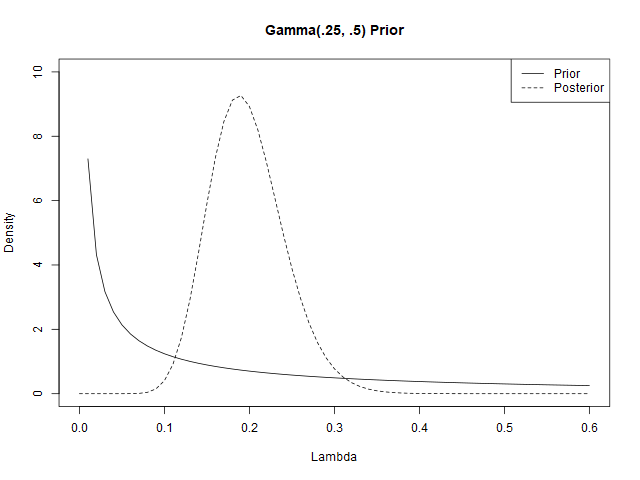
\includegraphics[scale = .5]{output/Problem62Plot_a.png}

The second prior has $\alpha = .25$ and $\beta = .025$. Thus the posterior is distributed $Gamma(20.25, 102.025)$ with a mean of $E(\Lambda|\sum_{i=1}^{20} X_i = 102) = 0.1656$.

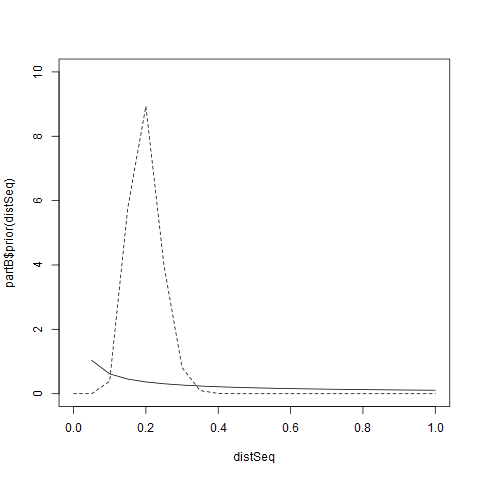
\includegraphics[scale = .5]{output/Problem62Plot_b.png}

Although the second prior is flatter, the differences are insignificant compared to the data.

\end{document}